\cleardoublepage
\chapter{Neurophysiological and behavioral factors associated with a high DRF}
\label{disc:drf}

\section{Summary of the results}
\label{disc:drf:summary}

\begin{figure}[htb]
	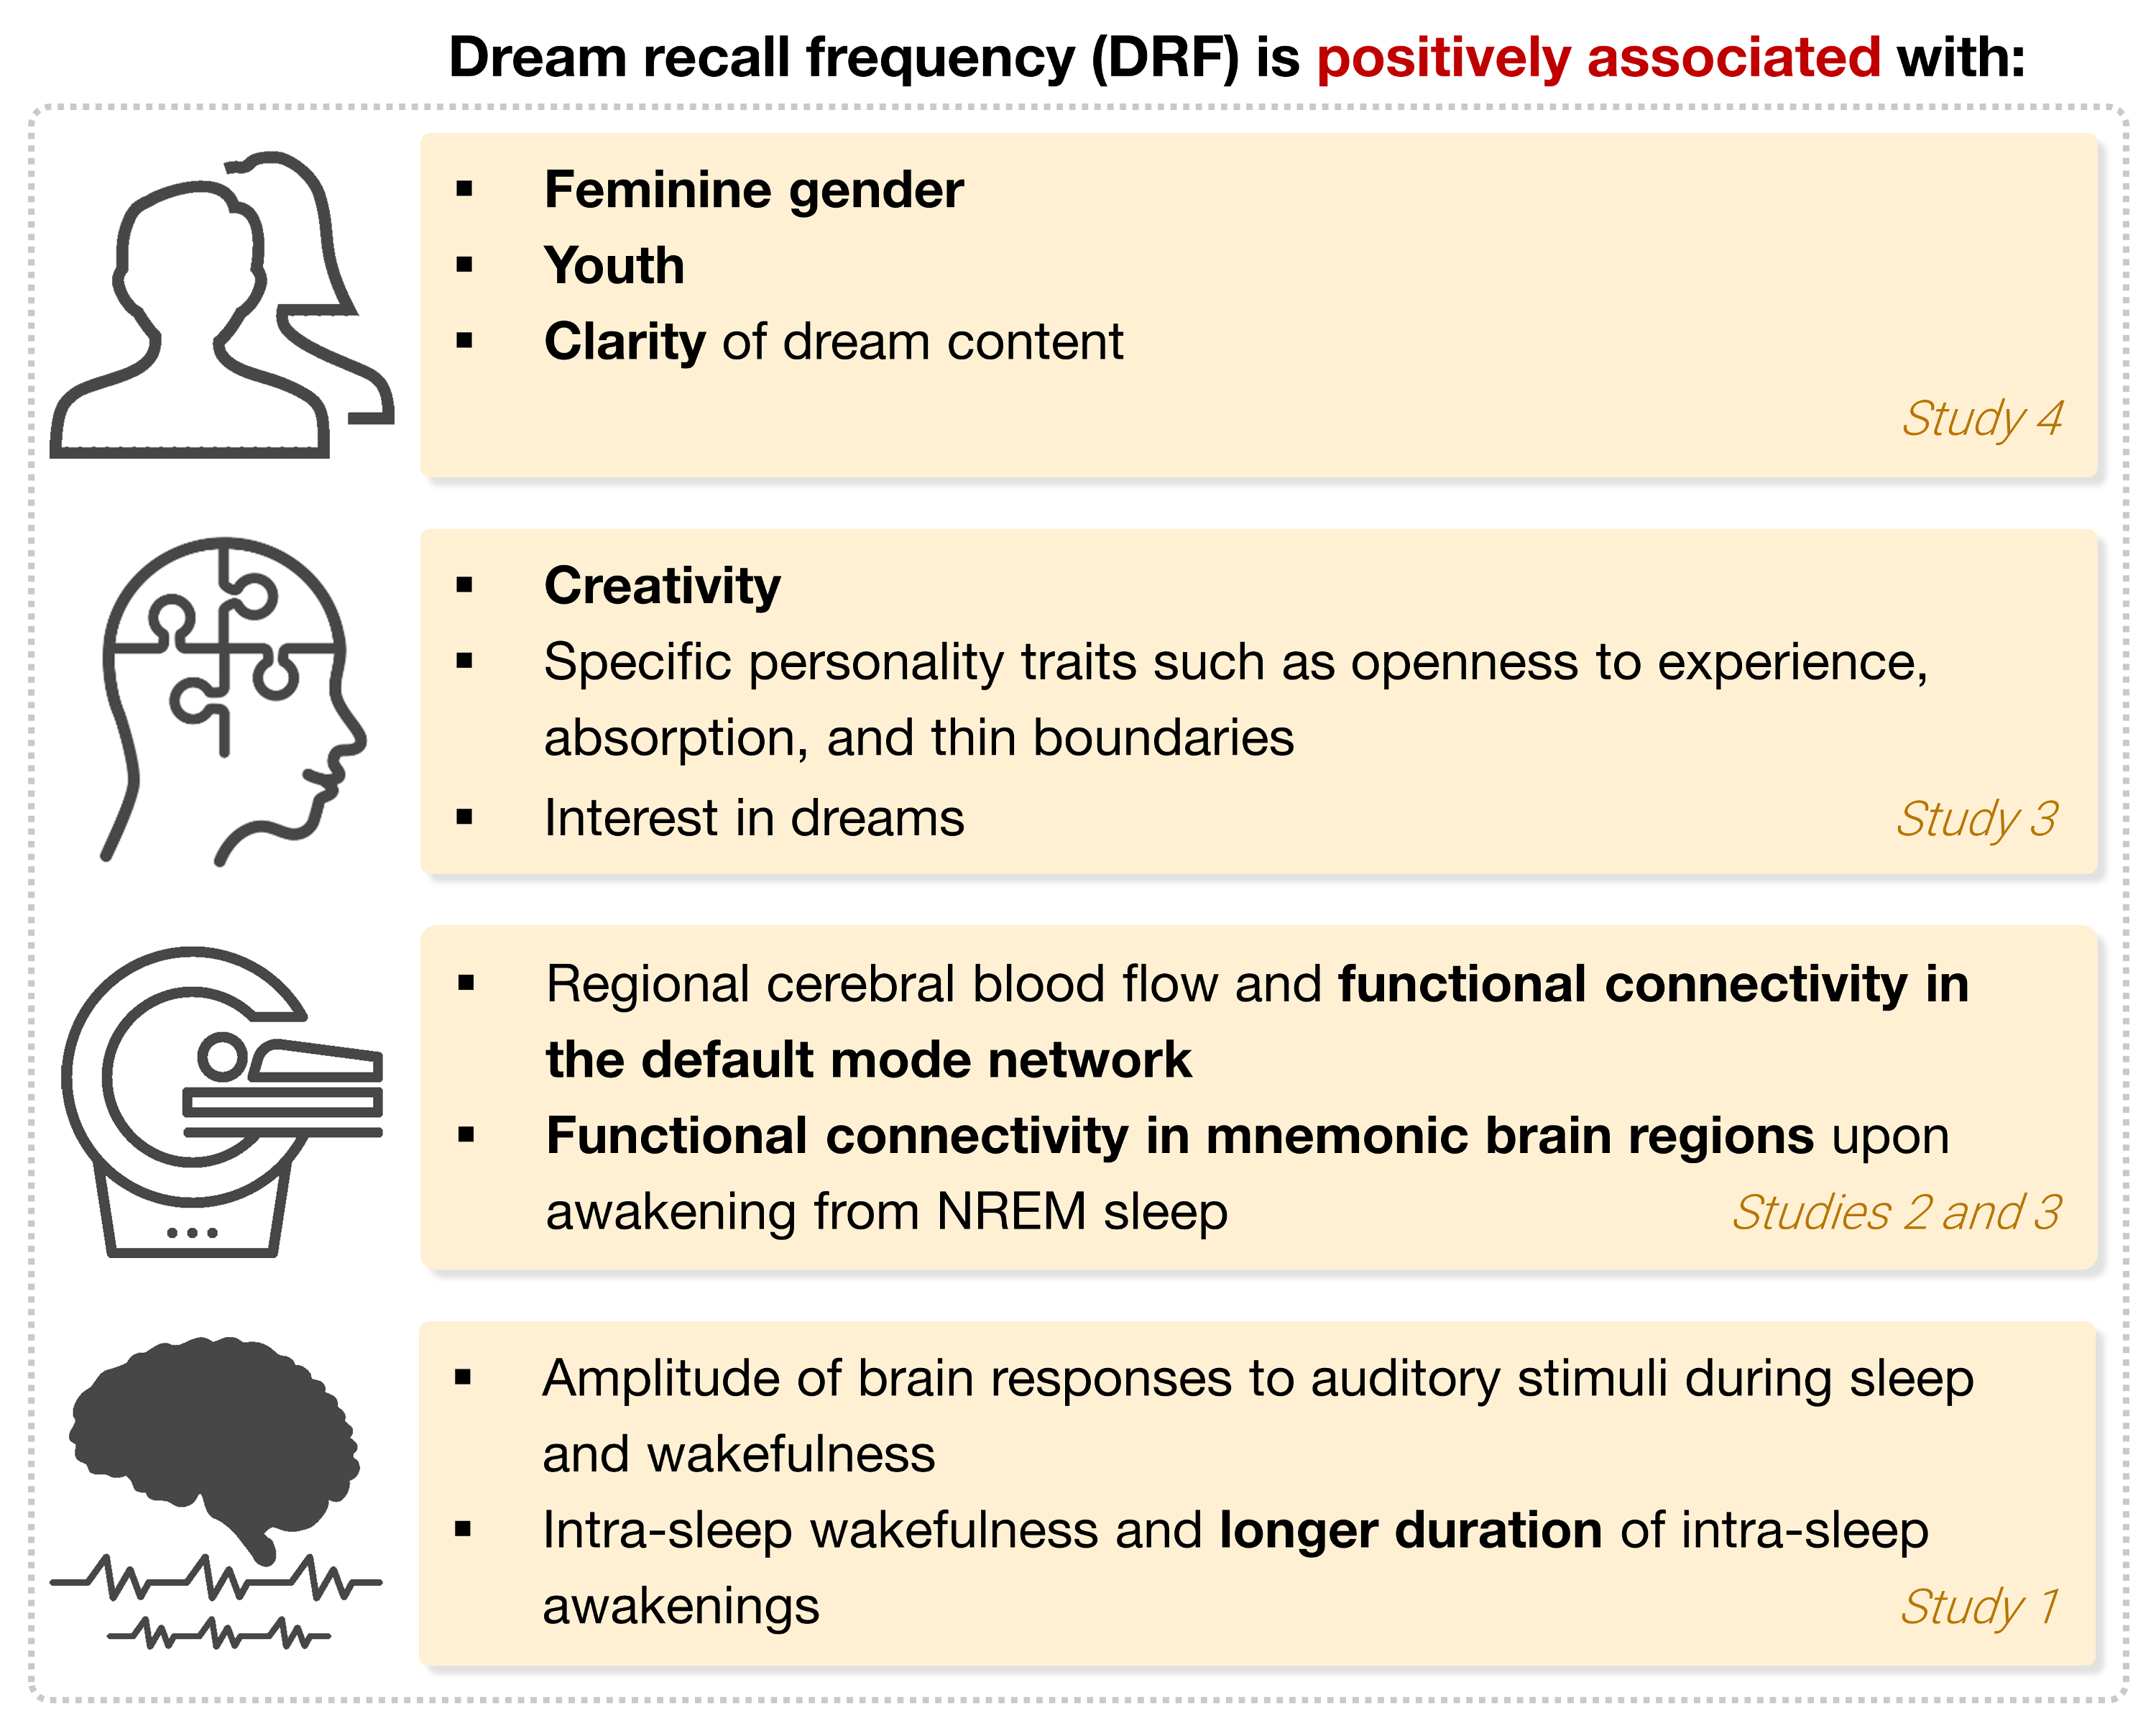
\includegraphics[width=\textwidth]{Fig/Discussion/HR_recap.png}
	\caption[Summary of the results on DRF]{Summary of the behavioral and neurophysiological differences observed between high and low dream recallers}
	\label{fig:disc:drf:summary}
\end{figure}


%%%%%%%%%%%%%%%%%%%%%%%%%%%%%%%%%%%%%%%%%%%%%%%%%%%%%%%%%%%%%%%%%%%%%%%%%%%%%%%
\cleardoublepage
\chapter{The relationship between waking life and dream content}
\label{disc:wle}

%%%%%%%%%%%%%%%%%%%%%%%%%%%%%%%%%%%%%%%%%%%%%%%%%%%%%%%%%%%%%%%%%%%%%%%%%%%%%%%
\cleardoublepage
\chapter{Methodological development}
\label{disc:methods}

\section{A state-of-the-art open-source software}
\label{disc:methods:software}



\section{Future directions}
\label{disc:methods:future}

\subsection{Automatic sleep scoring}
\label{disc:methods:future:auto}

\begin{figure}[htb]
	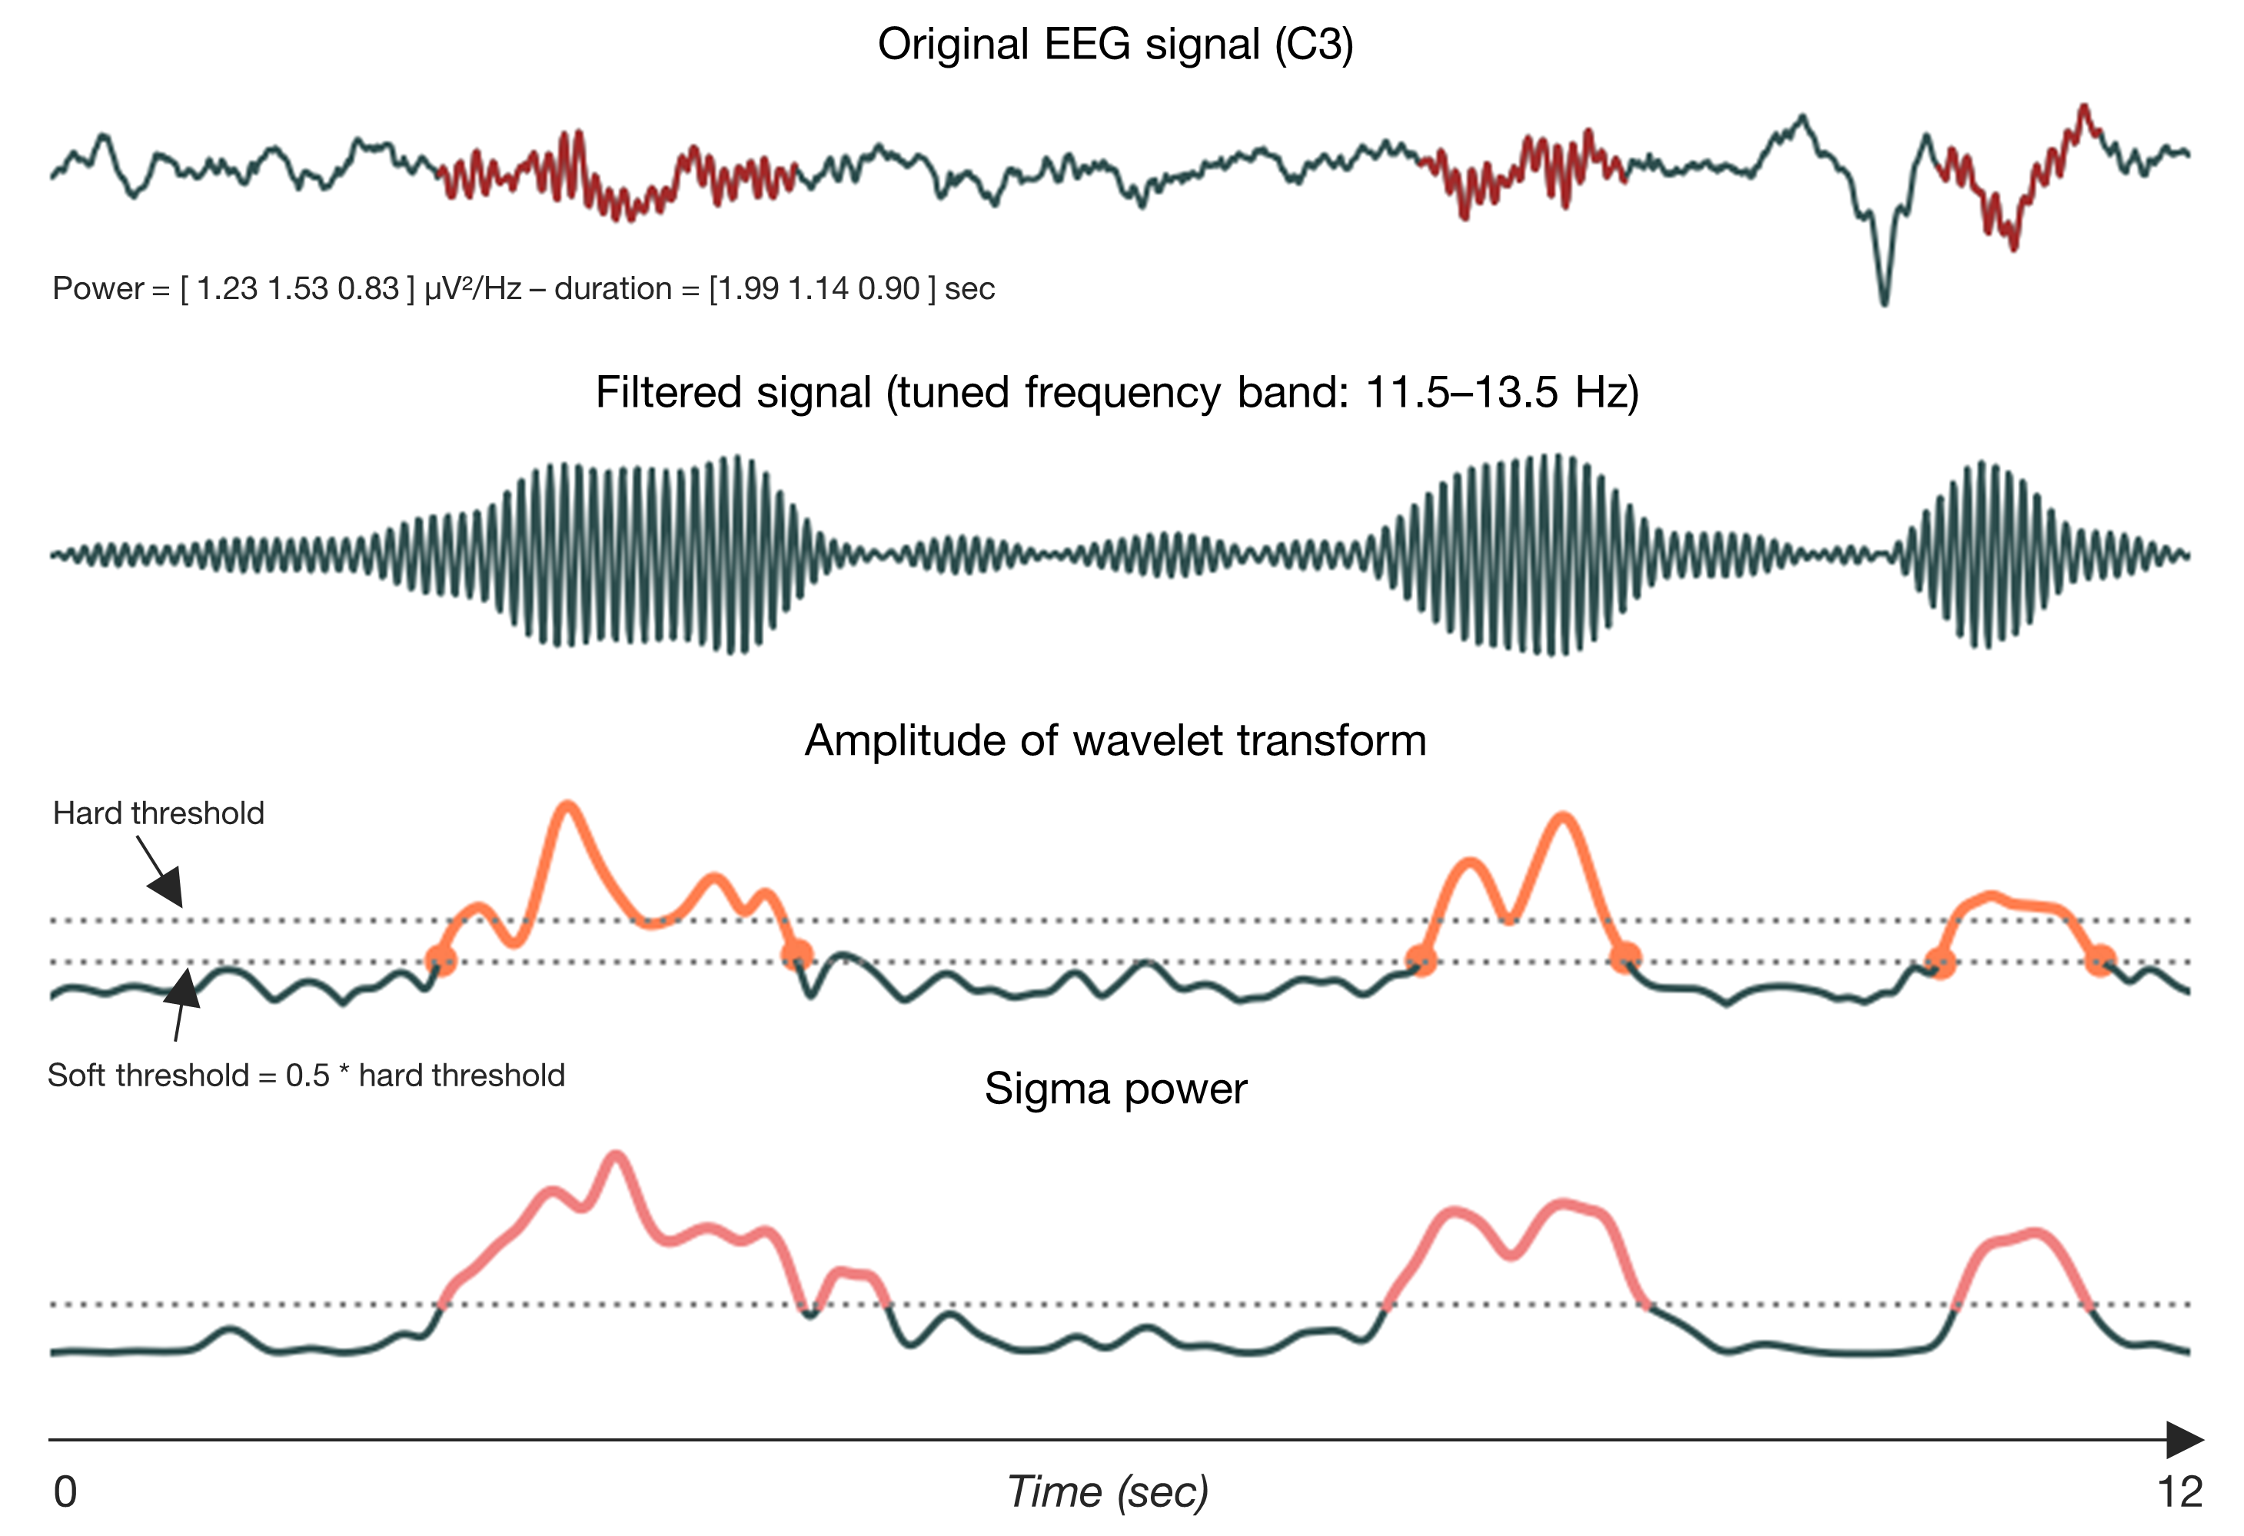
\includegraphics[width=\textwidth]{Fig/Discussion/spindles.png}
	\caption[Improved spindles detection and visualization]{Improved spindles detection and visualization within the software. Compared to the initial algorithm (presented in chapter \ref{res:software}), the new spindles detection has several improvements. First, we implemented a data-driven tuning of the spindle frequency band by finding the peak spectral power within the sigma range. This step, initially described by \citet{berthomier_automatic_2007}, allows to accommodate for inter-individual variability of EEG signals, and is particularly useful when analyzing patients who tend to exhibit higher variability. Second, we now use both a hard and a soft threshold on the amplitude of the wavelet transform to determine more precisely the beginning and the end of each spindle. Finally, to allow users to better understand how the detection algorithm works, we implemented a function to plot the current figure for each desired time window.}
	\label{fig:disc:methods:future:auto:spindles}
\end{figure}

\begin{figure}[htb]
	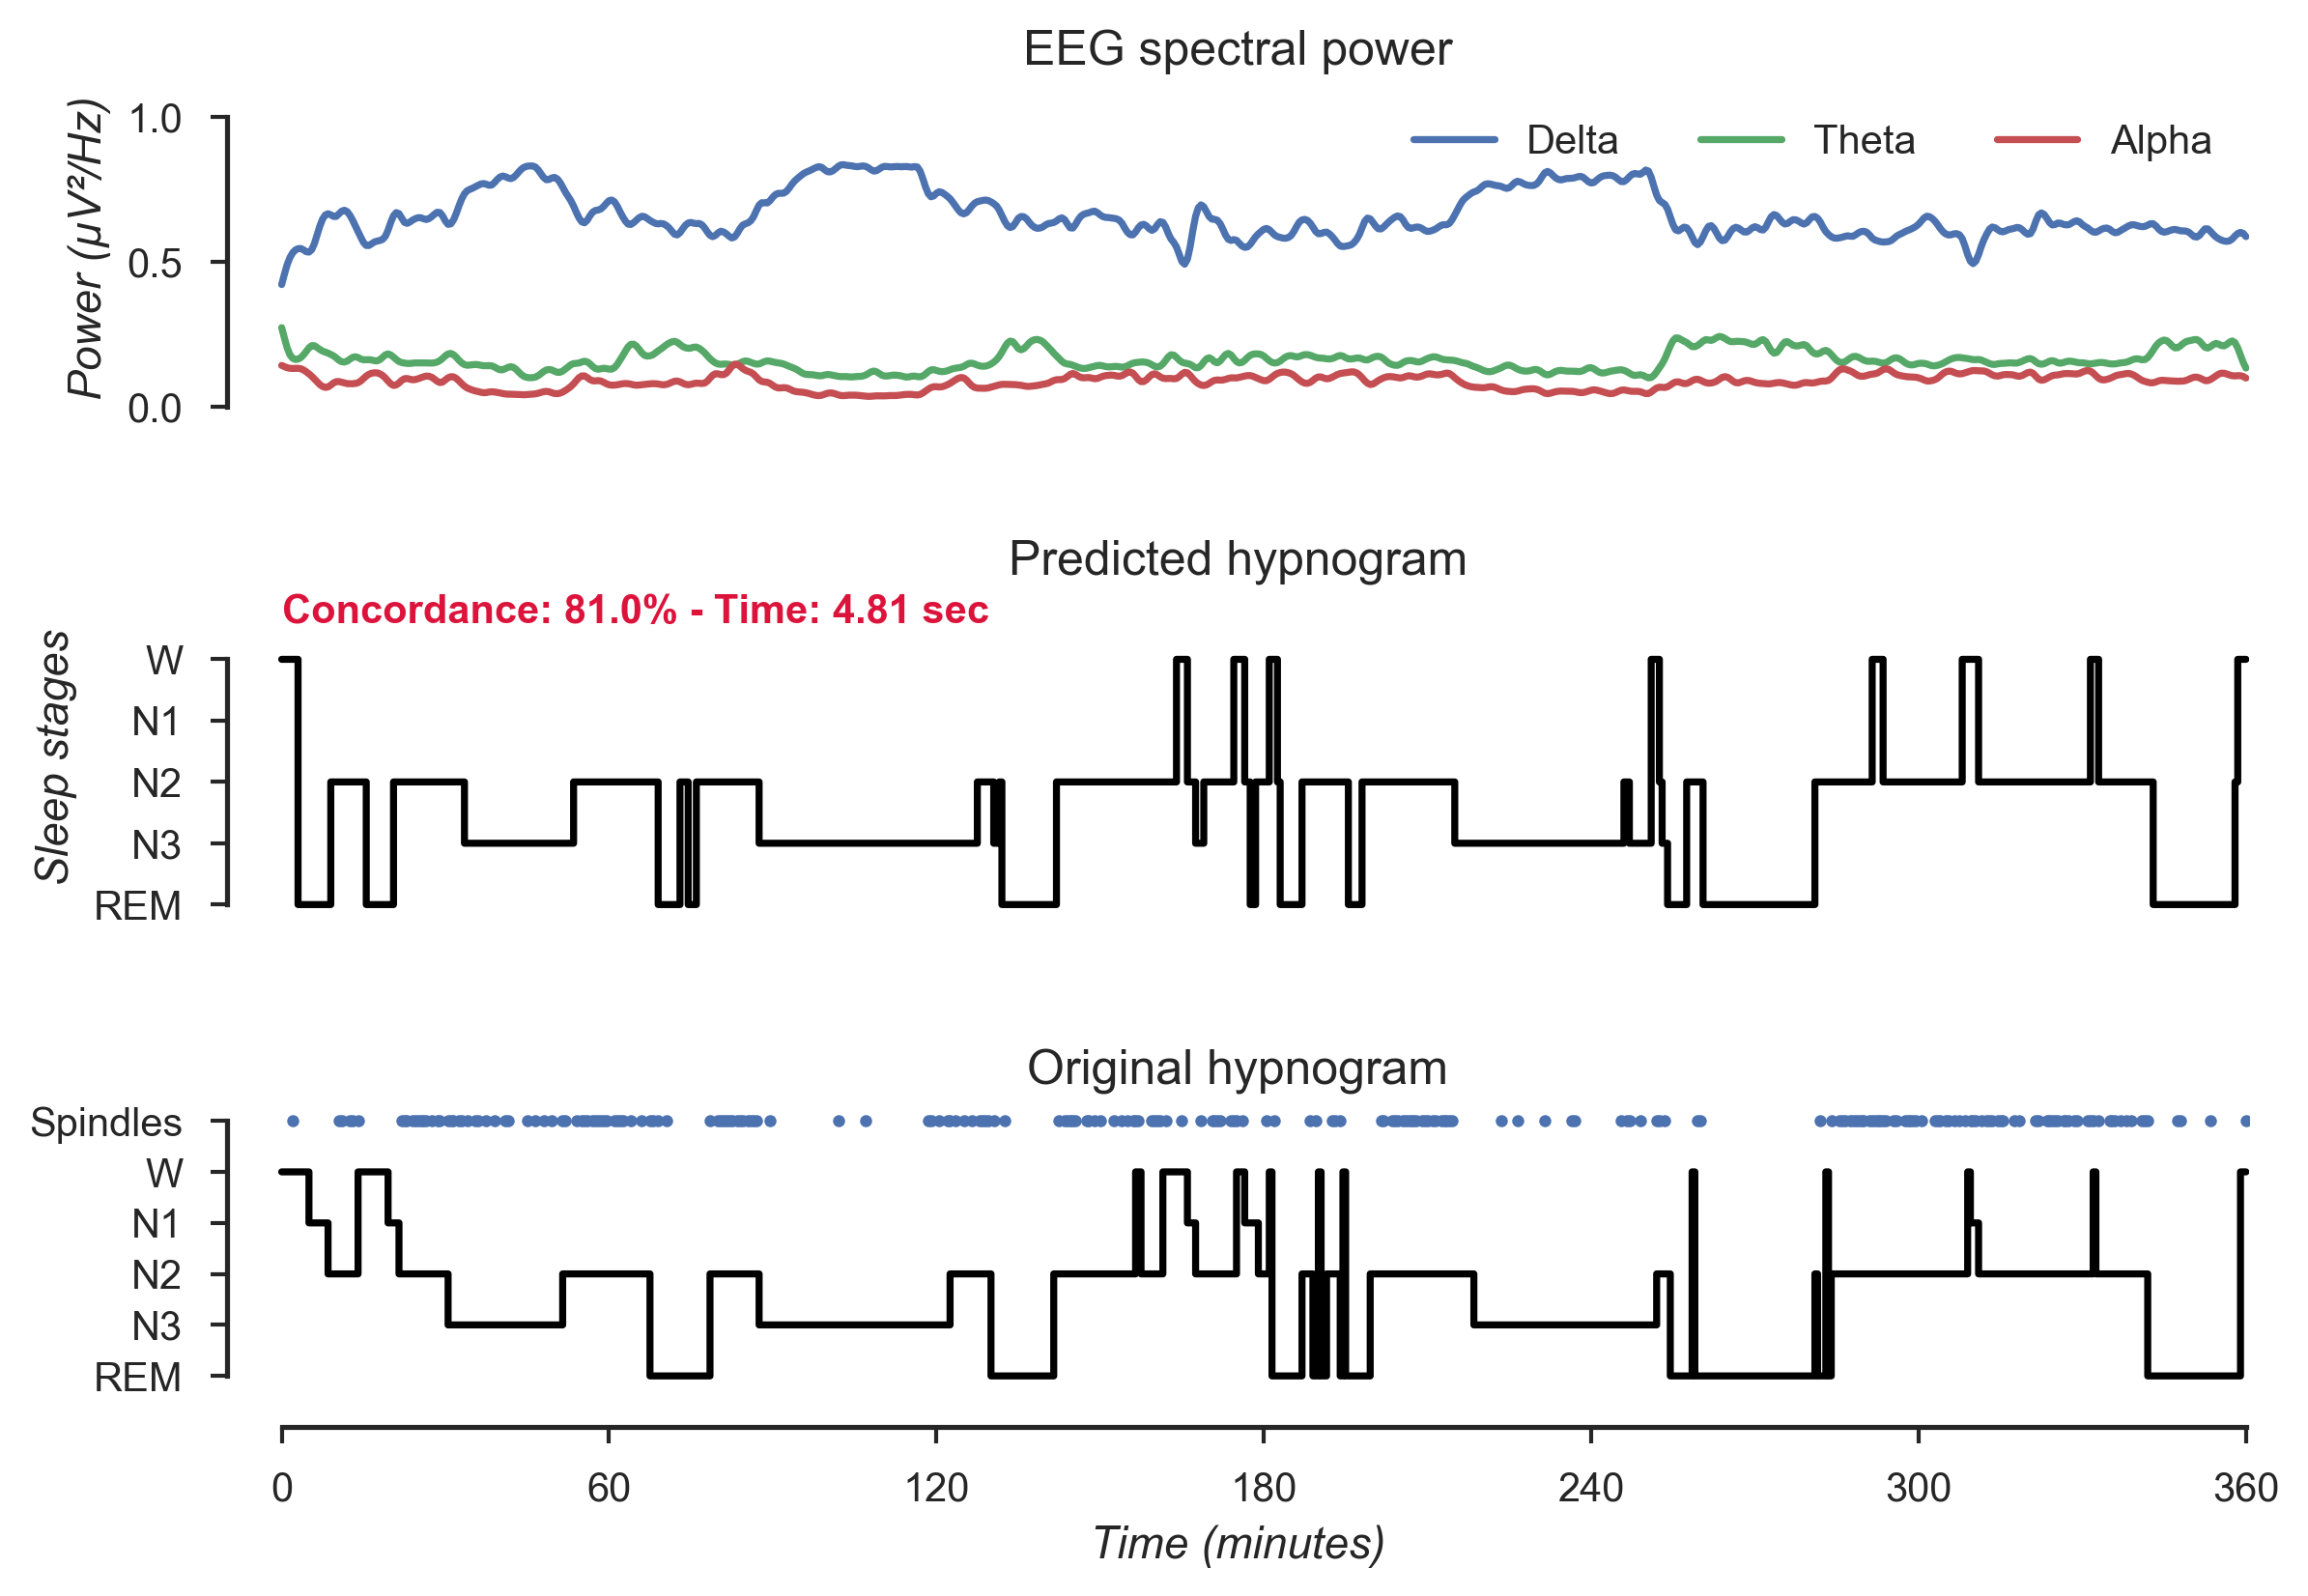
\includegraphics[width=\textwidth]{Fig/Discussion/autoscore.png}
	\caption[]{CAPTION TO DO}
	\label{fig:disc:methods:future:auto:autoscore}
\end{figure}


%%%%%%%%%%%%%%%%%%%%%%%%%%%%%%%%%%%%%%%%%%%%%%%%%%%%%%%%%%%%%%%%%%%%%%%%%%%%%%%
\cleardoublepage
\chapter{General conclusion}
\label{disc:conclusion}
